% quant_guide.tex -- beginner guide to the fx-var-normality-test project
% Compile from inside the docs/ folder:
%   pdflatex quant_guide && bibtex quant_guide && pdflatex quant_guide && pdflatex quant_guide
\documentclass[11pt,a4paper]{article}

\usepackage[T1]{fontenc}
\usepackage[utf8]{inputenc}
\usepackage{lmodern}
\usepackage{microtype}
\usepackage[margin=2.5cm]{geometry}
\usepackage{amsmath,amssymb}
\usepackage{graphicx}
\usepackage{booktabs}
\usepackage{enumitem}
\usepackage[most]{tcolorbox}
\usepackage{tikz}
\usepackage[authoryear,round]{natbib}
\usepackage[hidelinks,pdfauthor={Hugo Johansson},pdftitle={Guideline for Noobs}]{hyperref}

\graphicspath{{../figures/}}
\setlength{\parindent}{0pt}
\setlength{\parskip}{0.6em}
\setlist{itemsep=0.2em}

% ---------- Boxes ----------
\newtcolorbox{onesentence}{colback=blue!4,colframe=blue!50!black,
  fonttitle=\bfseries,title={In one sentence},breakable}
\newtcolorbox{example}[1][]{colback=green!4,colframe=green!40!black,
  fonttitle=\bfseries,title={Example#1},breakable}
\newtcolorbox{mistake}{colback=red!4,colframe=red!55!black,
  fonttitle=\bfseries,title={Common mistake},breakable}
\newtcolorbox{fictive}{colback=orange!6,colframe=orange!70!black,
  fonttitle=\bfseries,title={Fictive story -- made-up numbers},breakable}

% ---------- Glossary entry helpers ----------
\newcommand{\term}[1]{\subsection{#1}}
\newcommand{\plain}{\textbf{In plain words.} }
\newcommand{\inproj}{\textbf{In the project.} }
\newcommand{\tinyex}{\textbf{Tiny example.} }

\newcommand{\code}[1]{\texttt{#1}}

\title{Guideline for Noobs}
\author{Hugo Johansson}
\date{October 2026}

\begin{document}

\begin{titlepage}
    \centering
    \vspace*{0.5cm}

    {\large\scshape a friendly guide to}\\[0.6cm]
    \rule{\linewidth}{0.5mm}\\[0.5cm]
    {\fontsize{34}{40}\selectfont\bfseries Guideline for Noobs}\\[0.4cm]
    {\Large Quant finance, risk and the EUR/USD project}\\[0.2cm]
    {\large explained like you are curious, not like you are an expert}\\[0.5cm]
    \rule{\linewidth}{0.5mm}

    \vspace{1cm}

    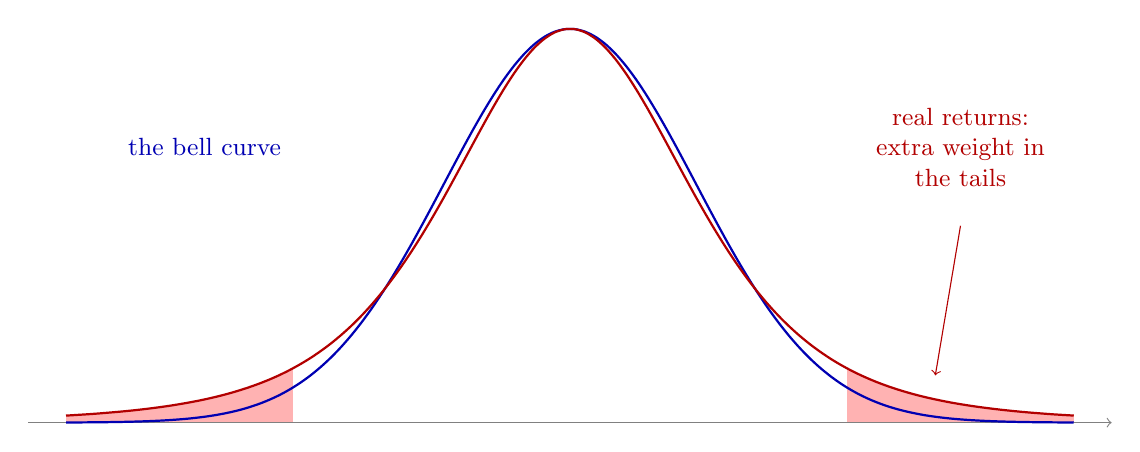
\begin{tikzpicture}[x=1.6cm,y=5cm]
      \fill[red!30] (2.2,0) -- plot[domain=2.2:4,samples=40] (\x,{(1+\x*\x/4)^(-2.5)}) -- (4,0) -- cycle;
      \fill[red!30] (-2.2,0) -- plot[domain=-2.2:-4,samples=40] (\x,{(1+\x*\x/4)^(-2.5)}) -- (-4,0) -- cycle;
      \draw[->,gray] (-4.3,0) -- (4.3,0);
      \draw[thick,blue!70!black,domain=-4:4,smooth,samples=100]
        plot (\x,{exp(-\x*\x/2)});
      \draw[thick,red!70!black,domain=-4:4,smooth,samples=100]
        plot (\x,{(1+\x*\x/4)^(-2.5)});
      \node[blue!70!black,font=\small] at (-2.9,0.7) {the bell curve};
      \node[red!70!black,font=\small,align=center] at (3.1,0.7)
        {real returns:\\extra weight in\\the tails};
      \draw[->,red!70!black] (3.1,0.5) -- (2.9,0.12);
    \end{tikzpicture}

    \vfill

    \begin{tcolorbox}[colback=gray!8,colframe=gray!50,width=0.88\textwidth,
        arc=3mm,boxrule=0.4pt]
      \small
      \textbf{Hi, I'm Hugo.} I like statistics, probability and programming,
      but I am \emph{not} an advanced quant. I wrote this guide to learn,
      so I explain every idea the way I wish someone had explained it to me:
      small examples first, formulas second. If something here is
      unclear, that is a bug in the guide, not in you.
    \end{tcolorbox}

    \vspace{0.6cm}

    {\Large\bfseries Hugo Johansson}\\[0.2cm]
    {\large October 2026}

    \vfill

    \begin{minipage}{0.85\textwidth}
        \centering
        \scriptsize \textit{Declaration of AI use. The author of this guide is
        Hugo Johansson, who takes full responsibility for the content and the
        final version. The code, the guide and the literature search were
        produced with Claude Sonnet 5.5 (Anthropic) and a number of Claude
        sub-agents (a research agent for the sources and a writing agent for
        the guide). The code and the guide were afterwards reviewed by two
        other AI systems, Gemini (Google) and ChatGPT (OpenAI). AI review
        does not replace checking by the author; see \texttt{AI\_USE.md} in
        the repository for a task-by-task log.}
    \end{minipage}
\end{titlepage}

\thispagestyle{empty}
\newpage
\setcounter{page}{1}

\begin{center}
\small\itshape This guide is for learning only. It is not investment advice,
and nothing in it says where EUR/USD is going.
\end{center}

\tableofcontents
\newpage

%=====================================================================
\section{How to use this guide}
%=====================================================================

This guide explains the words and ideas behind my GitHub project
\emph{fx-var-normality-test}. The project asks two questions:

\begin{enumerate}
  \item Are daily EUR/USD returns normally distributed?
  \item If we pretend they are, do we underestimate the risk?
\end{enumerate}

The short answers are ``no'' and ``yes, at the 99\% level''. The rest of
this guide explains what those answers mean.

\textbf{Who is this for?} A first-year student who knows some basic Python
and has seen a Monte Carlo simulation, but has not studied quant finance.
If you can write a \code{for} loop and you know what an average is, you are
ready.

\textbf{How is it built?}
\begin{itemize}
  \item \textbf{Part A} (Section~\ref{sec:glossary}) is a glossary
    (\emph{begreppslista}). Every word gets a plain definition, a tiny example
    with numbers, and a note on where it shows up in the project. Use it like
    a dictionary. You do not have to read it from top to bottom.
  \item \textbf{Part B} (Section~\ref{sec:project}) walks through the project
    step by step, with the real results.
  \item \textbf{Part C} (Section~\ref{sec:macro}) is about how exchange rates
    move with the economy, told as a made-up story where we trade EUR/USD.
  \item Then come limitations, exercises with answers, a one-page cheat
    sheet of formulas, and the references.
\end{itemize}

\textbf{The boxes.} Three kinds of boxes appear again and again:

\begin{onesentence}
The shortest possible version of an idea. If you only read these, you still
get the main points.
\end{onesentence}

\begin{example}
A small calculation with easy numbers, so you can check it on paper or in
Python.
\end{example}

\begin{mistake}
A trap that beginners (including me) fall into.
\end{mistake}

\textbf{A rule for the whole guide.} When I say something about what
researchers have found, there is a reference in brackets, like
\citep{jorion2007}. When there is no reference, it is either a definition,
a calculation you can check yourself, or my own reasoning, and I try to say
which. Numbers from the project come from running \code{var\_eurusd.py} on
ECB data from 4 January 1999 to 7 October 2026.

%=====================================================================
\section{Part A: Glossary (begreppslista)}\label{sec:glossary}
%=====================================================================

The terms are grouped so that each one only uses words that came before it.

%---------------------------------------------------------------------
\subsection*{A1. Prices, returns and the EUR/USD quote}
\addcontentsline{toc}{subsection}{A1. Prices, returns and the EUR/USD quote}
%---------------------------------------------------------------------

\term{EUR/USD quote convention}\label{g:quote}
\plain ``EUR/USD $= 1.1177$'' means \emph{one euro costs 1.1177 US dollars}.
The euro is the thing being priced; the dollar is the money we pay with.
So when the number goes \emph{up}, the euro has become \emph{stronger}
(you need more dollars to buy one euro). A rate going up gives a
\emph{positive} return.

\begin{example}
Monday EUR/USD is 1.10, Tuesday it is 1.12. One euro now buys 2 more US
cents. The euro got stronger, the dollar got weaker, and the return is
positive.
\end{example}

\inproj The ECB series \code{D.USD.EUR.SP00.A} gives how many dollars one
euro costs. The last value in the data is 1.1177. All returns in the project
are from the point of view of someone who \emph{holds euros and counts their
money in dollars}. For that person, a negative return is a loss.

\begin{mistake}
Mixing up the direction. ``EUR/USD fell'' means the \emph{euro} fell, not the
dollar. If you hold dollars and count in euros, a fall in EUR/USD is good
news for you.
\end{mistake}

\term{ECB reference rate}\label{g:ecb}
\plain Every working day the European Central Bank publishes one official
EUR/USD number. It is a snapshot taken in the early afternoon (the ECB's
page says around 14:10 CET; the data file itself labels it 2.15 pm CET) and
published around 16:00 CET \citep{ecbrefrates}. The ECB says the rates are for information,
not for doing trades \citep{ecbrefrates}.

\tinyex On a given day the market price moves thousands of times, but the ECB
data file contains just one number for that day, for example 1.1177.

\inproj The script downloads this series. Because it is one number per day,
we cannot see moves inside the day, and there is no bid/ask spread (the
small gap between buying and selling price a bank would charge you).

\term{Price vs return}\label{g:return}
\plain A \emph{price} is a level (``1.10 dollars per euro''). A
\emph{return} is a change, in percent (``up 2\% since yesterday''). Risk
models work with returns, because a 1-cent move means very different things
if the price is 1 dollar or 100 dollars.

\begin{example}
A price goes from 100 to 110. The simple return is
$(110-100)/100 = 10\%$. A price going from 1.00 to 1.10 also has a 10\%
return, even though it moved only 0.10.
\end{example}

\inproj The data contains prices (rates). The first thing the script does is
turn them into returns: 7109 prices give 7108 returns.

\term{Log return}\label{g:logreturn}
\plain A log return is a different way to measure the change:
\[
  r_t = 100 \cdot \ln\!\left(\frac{P_t}{P_{t-1}}\right) \quad \text{(in percent).}
\]
For small changes it is almost the same as the simple return. Its big
advantage: log returns \emph{add up}. The log return over two days is the
sum of the two daily log returns.

\begin{example}
Prices: 100, 110, 99.
\begin{itemize}
  \item Day 1: $100\ln(110/100) = +9.53\%$.
  \item Day 2: $100\ln(99/110) = -10.54\%$.
  \item Sum: $-1.01\%$, which is exactly $100\ln(99/100)$, the total change.
\end{itemize}
With simple returns you get $+10\%$ and $-10\%$. They add up to $0\%$, but
the price actually fell from 100 to 99. Simple returns do not add up; log
returns do.
\end{example}

\inproj \code{log\_returns(rates)} computes
\code{100 * np.diff(np.log(rates))}. The 2040 scenario uses the adding-up
property: it adds daily log returns and then uses \code{np.exp} to get back
to a price.

\begin{mistake}
Forgetting the factor 100. Then a ``1.3'' VaR would be read as 1.3 (that is
130\%) instead of 1.3\%.
\end{mistake}

\term{Mean}\label{g:mean}
\plain The average. Add everything up and divide by how many numbers there
are. Written $\mu$ (``mu'').

\tinyex Returns $+1, -1, +2, -2, +5$: mean $= 5/5 = 1\%$.

\inproj The mean daily EUR/USD log return over 1999--2026 is about
$-0.0008\%$. That is basically zero. Over one day, the direction is close to
a coin flip, and the size of the moves matters much more than the average.

\term{Standard deviation}\label{g:std}
\plain How far the numbers typically are from the mean. Written $\sigma$
(``sigma''). Steps: subtract the mean, square, average, take the square root.
\[
  \sigma = \sqrt{\frac{1}{n}\sum_{t=1}^{n}(r_t - \mu)^2}.
\]

\begin{example}
Returns $1, -1, 2, -2$. Mean $=0$. Squares: $1, 1, 4, 4$. Average of squares
$= 10/4 = 2.5$. Square root: $\sigma \approx 1.58\%$.
\end{example}

\inproj The daily standard deviation is about $0.58\%$. Note that
\code{np.std} divides by $n$, not $n-1$. With 500 or 7108 numbers the
difference is tiny.

\term{Volatility}\label{g:vol}
\plain In finance, ``volatility'' usually means the standard deviation of
returns. High volatility = big swings. Think of it as how ``stormy'' the
market is. Careful: there are several versions. \emph{Sample (historical)
volatility} is the standard deviation of past returns, as here.
\emph{Annualised volatility} rescales it to one year. \emph{Conditional
volatility} is the volatility on one particular day given what happened
before, and it can change from day to day (GARCH models, below). A
\emph{forecast volatility} is a prediction of the future.

\tinyex Daily volatility $0.58\%$ is a standard deviation: moves of roughly that
size are common. (It is not the same as the average absolute move, which is
a bit smaller for a bell curve, about $0.8\sigma$.) A rough yearly number is
$0.58\% \times \sqrt{252} \approx 9\%$ (this square-root-of-time rule assumes
independent days).

\inproj Volatility is the $\sigma$ in the normal VaR formula, estimated
from the last 500 days.

%---------------------------------------------------------------------
\subsection*{A2. Distributions and their shape}
\addcontentsline{toc}{subsection}{A2. Distributions and their shape}
%---------------------------------------------------------------------

\term{Normal distribution}\label{g:normal}
\plain The famous bell curve. It is completely described by two numbers:
the mean $\mu$ and the standard deviation $\sigma$. About 68\% of values are
within $1\sigma$ of the mean, about 95\% within $2\sigma$, and almost all
(99.7\%) within $3\sigma$. Very large values are \emph{extremely} rare.

\begin{example}
Heights of adults are close to normal. If the mean is 175 cm and
$\sigma=7$ cm, someone 196 cm tall is $3\sigma$ above the mean: rare but you
have seen it. Someone $8\sigma$ tall (231 cm) basically never exists.
\end{example}

\inproj The normal VaR and the Monte Carlo VaR assume that returns are
normal. The project tests if that is true. (Spoiler: no.)

\term{Skewness}\label{g:skew}
\plain Is the distribution lopsided? Skewness 0 means symmetric, like the
normal. Negative skew means a longer tail of big \emph{losses}; positive
skew means a longer tail of big \emph{gains}.

\tinyex A lottery ticket: you usually lose a little, and very rarely win a lot.
That is strong positive skew.

\inproj The skewness of EUR/USD returns is about $0.05$, very close to zero.
So the up moves and down moves are roughly mirror images. The problem with
normality is not the skew, it is the kurtosis.

\term{Kurtosis and excess kurtosis}\label{g:kurt}
\plain Kurtosis measures how much of the action is in the \emph{tails}
(the rare, extreme values). A normal distribution has kurtosis 3. Because
everyone compares with the normal, people use \emph{excess} kurtosis
$=$ kurtosis $-\,3$. So a normal has excess kurtosis 0.

\begin{example}
Picture two dice games that both have the same average and the same
standard deviation. Game A is mostly middle results. Game B is mostly very
small moves, but now and then a huge one. Game B has higher kurtosis: quiet
most of the time, with sudden shocks.
\end{example}

\inproj \code{stats.kurtosis} in SciPy returns \emph{excess} kurtosis by
default. For EUR/USD it is $3.31$, so the kurtosis is about $6.31$. That is
clearly more than a normal.

\begin{mistake}
Reading SciPy's ``3.31'' as ``kurtosis is about 3, so it is normal''. SciPy
already subtracted 3. The normal value is 0, not 3.
\end{mistake}

\term{Fat tails}\label{g:fattails}
\plain ``Fat tails'' (or heavy tails) means extreme values happen much more
often than the normal distribution says. Financial returns are well known
for this \citep{mandelbrot1963,fama1965,cont2001}, and daily exchange rates
too \citep{baillie1989}.

\begin{example}
The worst daily EUR/USD log return in the data is about $-4.7\%$
(19 December 2008). With $\sigma = 0.58\%$ that is about $8\sigma$. Under a
normal distribution the chance of a day that bad is about $2 \times
10^{-16}$, less than one in a trillion. We have only about 7100 days of
data, yet it happened. One extreme day alone does not prove fat tails, but
together with the excess kurtosis, the QQ plot and the Jarque--Bera test
below, the evidence against a thin-tailed normal model is strong.
\end{example}

\inproj Fat tails are why the normal VaR at 99\% is too low.

\term{QQ plot}\label{g:qq}
\plain A picture that compares your data with a normal distribution. Sort
your returns from smallest to largest. Next to each one, put the value a
normal distribution would ``expect'' at that rank. Plot one against the
other. If the data are normal, the points lie on a straight line. If the ends
bend away from the line, the tails are fatter (or thinner) than normal.

\tinyex If you have 100 returns, the 1st smallest should be near the normal's
1\% point (about $\mu - 2.33\sigma$). If your smallest return is instead
$\mu - 4\sigma$, that point sits far below the line.

\inproj Figure~\ref{fig:qq} (\code{figures/qq\_plot.png}), made with
\code{stats.probplot}. The middle follows the line, the two ends bend away:
an S-shape, the classic sign of fat tails.

%---------------------------------------------------------------------
\subsection*{A3. Testing ideas with data}
\addcontentsline{toc}{subsection}{A3. Testing ideas with data}
%---------------------------------------------------------------------

\term{Hypothesis test and p-value}\label{g:pvalue}
\plain A hypothesis test is a fair way to ask ``could this just be bad
luck?''. You start with a boring assumption, the \emph{null hypothesis}
$H_0$ (``the coin is fair'', ``returns are normal''). Then you compute how
surprising your data would be \emph{if $H_0$ were true}. That surprise
level is the p-value: the probability of getting data at least this extreme
when $H_0$ is true. A small p-value (usual cutoff: $0.05$) means ``too
surprising, I reject $H_0$''.

\begin{example}
You flip a coin 10 times and get 10 heads. If the coin is fair, the chance
of that is $0.5^{10} \approx 0.001$. That p-value is tiny, so you reject
``the coin is fair''. If you got 6 heads, the p-value would be large and
you would not reject.
\end{example}

\inproj Two tests use p-values: Jarque--Bera (are returns normal?) and
Kupiec (does a VaR model break as often as it should?).

\begin{mistake}
Saying ``p $= 0.34$, so the model is proven correct''. A large p-value only
means ``no evidence against it''. It does not prove $H_0$ is true.
\end{mistake}

\term{Jarque--Bera test}\label{g:jb}
\plain A test of ``the data are normal'' that uses two numbers: skewness $S$
and excess kurtosis $K$. Both are 0 for a normal, so if either is far from
0 the statistic becomes large \citep{jarquebera1980,jarquebera1987}:
\[
  JB = \frac{n}{6}\left(S^2 + \frac{K^2}{4}\right) \sim \chi^2(2)
  \quad \text{if } H_0 \text{ is true (approximately, for large } n).
\]
The 5\% critical value of $\chi^2(2)$ is about 5.99. The $\chi^2(2)$
result is an approximation for large $n$, and it treats the observations as
independent. Daily returns show volatility clustering (below), so the exact
p-value should be taken with care. With a statistic this large, the
conclusion does not change.

\begin{example}
Suppose $n=600$, $S=0$ and $K=0.4$. Then
$JB = 100 \cdot (0 + 0.16/4) = 4$. That is below 5.99, so we do not reject
normality. If instead $K=1$, then $JB = 100 \cdot 0.25 = 25$, and we reject.
\end{example}

\inproj With $n=7108$, $S=0.05$ and $K=3.31$:
$JB = \tfrac{7108}{6}(0.0025 + 2.74) \approx 3244$. The p-value is
basically 0. Normality is clearly rejected.

\begin{mistake}
Thinking that a big $n$ makes the test ``unfair''. It is true that with
many days even a small deviation from normal is detected. But here the
deviation is not small: an excess kurtosis of 3.31 is large.
\end{mistake}

%---------------------------------------------------------------------
\subsection*{A4. Value-at-Risk}
\addcontentsline{toc}{subsection}{A4. Value-at-Risk}
%---------------------------------------------------------------------

\term{Value-at-Risk (VaR)}\label{g:var}
\plain A VaR answers: ``On a normal bad day, how much could I lose?'' More
exactly: the 99\% one-day VaR is a loss level that you expect to be beaten
on only 1\% of days \citep{jorion2007}. In the project it is written as a
\emph{positive} percentage loss.

\begin{example}
``The 99\% one-day VaR is 1.3\%.'' This means: on 99 days out of 100 you
should lose less than 1.3\%. On about 1 day in 100 (two or three days a
year) you lose more. If you hold euros worth 1{,}000{,}000 dollars, a 1.3\%
loss is 13{,}000 dollars.
\end{example}

\inproj Every day of the backtest, three methods compute a VaR at 95\% and
99\%.

\begin{mistake}
Thinking VaR is the \emph{worst} possible loss. It is not. VaR says nothing
about \emph{how big} the loss is on the 1\% bad days. That is a known
weakness; the measure ``expected shortfall'' looks at the average loss in
the tail instead \citep{artzner1999}.
\end{mistake}

\term{Confidence level}\label{g:level}
\plain The ``99\%'' or ``95\%'' in VaR. It says how often the VaR line should
hold. 99\% means ``broken 1 day in 100'', 95\% means ``broken 1 day in 20''.
A higher level means a line further out in the tail, so a bigger VaR number.

\tinyex It is like a flood wall. A wall built for the ``1 in 20 years''
flood is lower than a wall built for the ``1 in 100 years'' flood.

\inproj \code{LEVELS = [0.95, 0.99]}. The interesting level is 99\%,
because that is deep in the tail, where fat tails matter most.

\term{Parametric (normal) VaR}\label{g:varnormal}
\plain Assume returns are normal, estimate $\mu$ and $\sigma$, and read the
cutoff from the bell curve:
\[
  \text{VaR} = -(\mu + z\,\sigma), \qquad z = \Phi^{-1}(1-\text{level}),
\]
where $\Phi^{-1}$ is the inverse of the normal distribution function
(\code{stats.norm.ppf}). At 99\%, $z = \Phi^{-1}(0.01) \approx -2.326$; at
95\%, $z \approx -1.645$. Because $z$ is negative, $\mu + z\sigma$ is a
negative return (a loss), and the minus sign in front makes VaR positive.
This normal (``variance--covariance'') approach is the one described in the
RiskMetrics technical document \citep{riskmetrics1996}.

\begin{example}
Using the whole sample: $\mu = -0.0008\%$ and $\sigma = 0.581\%$.
99\% VaR $= -(-0.0008 + (-2.326)(0.581)) \approx 1.35\%$.
\end{example}

\inproj \code{var\_normal(window, level)}. Over the backtest, the average
99\% normal VaR is $1.32\%$.

\term{Historical VaR (historical simulation)}\label{g:varhist}
\plain Do not assume any shape. Take your past returns, sort them, and pick
the one that is 1\% from the bottom (for 99\%). ``The past is my
distribution.'' Its weaknesses are discussed by \citet{pritsker2006}.

\begin{example}
You have 500 past returns. 1\% of 500 is 5. So the 99\% VaR is roughly the
5th or 6th worst return (\code{np.quantile} interpolates between
neighbouring values). If the 5 worst days were $-2.1, -1.8, -1.6, -1.5,
-1.45\%$, the VaR would be about 1.45\%.
\end{example}

\inproj \code{var\_historical} uses \code{-np.quantile(window, 1 - level)}.
Average 99\% historical VaR in the backtest: $1.41\%$, higher than the
normal one, because the real tail is fatter than the bell curve.

\term{Monte Carlo VaR}\label{g:varmc}
\plain Simulate many fake returns from a model, then use the historical
method on the fake returns. In the project the model is a normal
distribution with the window's $\mu$ and $\sigma$.

\tinyex Draw 10{,}000 numbers from a normal with $\mu=0$, $\sigma=0.58$. The
100th smallest is close to $-2.326 \times 0.58 \approx -1.35$. So the
simulated VaR is close to the formula VaR.

\inproj \code{var\_monte\_carlo} with \code{N\_DRAWS = 10000}. Because it
uses the same normal assumption, it should land very close to the
parametric normal VaR, with a little simulation noise. In this particular
run the exceedance counts happen to be identical (114 and 302). Monte Carlo is only as good as the model you feed it.

\begin{mistake}
Thinking ``Monte Carlo'' automatically means ``more realistic''. A
simulation from a normal distribution still has thin normal tails.
\end{mistake}

%---------------------------------------------------------------------
\subsection*{A5. Checking a VaR model}
\addcontentsline{toc}{subsection}{A5. Checking a VaR model}
%---------------------------------------------------------------------

\term{Exceedance}\label{g:exceed}
\plain A day when the loss is bigger than the VaR. Also called a ``hit'',
``breach'' or ``violation''. In the project: $r_t < -\text{VaR}_t$.

\tinyex The VaR is like a speed limit and an exceedance is a speeding ticket.
A 99\% VaR should give about 1 ticket per 100 days. If you get 2 tickets
every 100 days, the limit is set wrong.

\inproj \code{n\_exceed = int(np.sum(test\_returns < -var\_values))}.

\term{Backtesting}\label{g:backtest}
\plain Pretend you are back in the past. Every day, compute the VaR using
only what you knew then, and see whether the next return broke it. Then
count the exceedances. Banking regulators use this idea to check banks'
VaR models \citep{basel1996backtesting}.

\tinyex With 1000 test days at 99\%, you expect about 10 exceedances. If you
see 25, the model is too optimistic. If you see 1, it is too cautious.

\inproj 6608 test days. At 99\% we expect $0.01 \times 6608 = 66.1$
exceedances.

\term{Rolling window}\label{g:window}
\plain Use only the last $W$ days to estimate the model, and move the window
forward one day at a time. Old data drop out, new data come in.

\tinyex $W=500$. To estimate the VaR for day 501, use days 1--500. For day
502, use days 2--501. And so on.

\inproj \code{WINDOW = 500} (about two years of working days), and
\code{window = returns[day - WINDOW:day]}.

\term{Look-ahead bias}\label{g:lookahead}
\plain Cheating by accident: using information that you could not have known
at the time. It makes a backtest look better than reality.

\begin{example}
You test a VaR for 15 September 2008, but your window includes data from
October 2008. Your model ``knows'' the crisis is coming. In real life it
could not.
\end{example}

\inproj The Python slice \code{returns[day - WINDOW:day]} stops \emph{before}
\code{day} (the end of a slice is not included). So the VaR for day
\code{day} only uses earlier returns.

\begin{mistake}
Writing \code{returns[day - WINDOW:day + 1]}. One extra day sounds harmless,
but it puts the very return you are testing into the window.
\end{mistake}

\term{Kupiec test}\label{g:kupiec}
\plain A test of ``the model breaks exactly as often as it promises''
\citep{kupiec1995}. With $n$ test days, $x$ exceedances and a target
rate $p$ (0.01 at 99\%), the test compares two likelihoods: how likely $x$
is if the true rate is $p$, and how likely it is if the true rate is the
observed $x/n$:
\[
  LR = -2\ln\!\left[\frac{(1-p)^{\,n-x}\,p^{\,x}}
       {\left(1-\frac{x}{n}\right)^{n-x}\left(\frac{x}{n}\right)^{x}}\right]
  \sim \chi^2(1) \quad \text{if } H_0 \text{ is true.}
\]
The 5\% critical value of $\chi^2(1)$ is about 3.84.

\begin{example}
One year: $n=250$ days, $p=0.01$, so we expect 2.5 exceedances. We see
$x=6$. Plugging in gives $LR \approx 3.56$ and a p-value of about 0.06. Just
above 0.05, so we (barely) do not reject. More than double the expected
number of breaks, and still not rejected: one year at 99\% is too short to
say much.
\end{example}

\inproj \code{kupiec\_test(n\_days, n\_exceed, p)}. The code works with
logs, so it adds $x\ln p$ instead of multiplying $p^x$, which avoids numbers
too small for the computer.

\begin{mistake}
Thinking ``few exceedances'' is always good. Too \emph{few} is also a
failure: the VaR is too high, and a bank would hold more capital than needed.
Kupiec rejects in both directions. Kupiec also does not check whether
exceedances come in clusters; that needs another test
\citep{christoffersen1998}.
\end{mistake}

%---------------------------------------------------------------------
\subsection*{A6. Simulation}
\addcontentsline{toc}{subsection}{A6. Simulation}
%---------------------------------------------------------------------

\term{Monte Carlo}\label{g:mc}
\plain Answer a question by simulating it many times with random numbers
and looking at the results \citep{glasserman2003}. Named after the casino.

\tinyex What is the chance that two dice sum to 7? Roll them 100{,}000 times
in Python and count. You get close to $6/36 \approx 16.7\%$.

\inproj Used twice: the Monte Carlo VaR (normal draws) and the 2040
scenarios (bootstrap draws). Both use \code{np.random.seed(42)}, so you get
the same numbers every run.

\term{Bootstrap}\label{g:bootstrap}
\plain A Monte Carlo method where you do not invent a distribution. Instead
you draw \emph{from your own data}, with replacement \citep{efron1979,
efrontibshirani1986}.

\begin{example}
Write each of the 7108 historical daily returns on a marble and put them all
in a bag. To simulate one future day, pull out a marble, write down the
number, and put it back. Repeat for every future day. Because the real
crash days are in the bag, the fat tails come along automatically.
\end{example}

\inproj The function \code{scenario\_to\_2040} does this with
\code{np.random.choice(returns, size=(n\_paths, n\_days))}.

\term{Scenario analysis vs forecast}\label{g:scenario}
\plain A \emph{forecast} says ``this is where I think it will be''. A
\emph{scenario analysis} says ``if the future behaves like this, here is the
range of things that could happen''. It is a map of possibilities, not a
prediction.

\tinyex ``Tomorrow will be 14 degrees'' is a forecast. ``In Stockholm in
October, the temperature is usually between 2 and 14 degrees'' describes a
range of scenarios. The second is useful for packing a suitcase, but it
does not tell you what tomorrow will be.

\inproj The fan chart to 2040 is a scenario analysis. Why I do not call it
a forecast is my own reasoning, explained in Part B: the model has no idea
about direction (the mean is about zero), and research shows that exchange
rates are very hard to forecast at all \citep{meese1983,rossi2013}.

%---------------------------------------------------------------------
\subsection*{A7. Volatility that changes over time}
\addcontentsline{toc}{subsection}{A7. Volatility that changes over time}
%---------------------------------------------------------------------

\term{Volatility clustering}\label{g:cluster}
\plain Calm days tend to follow calm days, and wild days tend to follow wild
days. Volatility comes in ``spells''. It is one of the best-known facts about
financial returns \citep{cont2001}.

\tinyex Like weather: if today is stormy, tomorrow is more likely to be stormy
than a random day in the year. Storms come in periods, not one isolated day
at a time.

\inproj You can see it in Figure~\ref{fig:varlines}: the grey returns are
much wider in 2008--2009 than in quiet years. The project does
\emph{not} model this. A 500-day window reacts slowly, and the bootstrap
draws days independently.

\term{Conditional heteroscedasticity}\label{g:condhet}
\plain A long name for a simple idea. ``Heteroscedasticity'' = the variance
is not constant. ``Conditional'' = the variance today depends on what
happened before (it is conditional on the past). Volatility clustering is
the pattern you can see in a chart, and it is consistent with a conditional
variance that changes over time.

\tinyex If yesterday's move was $-2\%$, our best guess for today's volatility
is higher than if yesterday's move was $+0.1\%$, even though we have no idea
about today's direction.

\inproj Not modelled. The normal VaR uses one $\sigma$ for the whole
500-day window, as if the variance were constant inside it.

\term{ARCH}\label{g:arch}
\plain ``AutoRegressive Conditional Heteroscedasticity'' \citep{engle1982}.
Today's variance is a constant plus a part of yesterday's \emph{squared}
surprise $\varepsilon_{t-1}$ (the return minus its mean):
\[
  \sigma_t^2 = \omega + \alpha\,\varepsilon_{t-1}^2 .
\]
Squared, because a big move \emph{in either direction} raises volatility.

\tinyex With $\omega=0.2$ and $\alpha=0.3$ (made-up numbers): after a $2\%$
move, $\sigma_t^2 = 0.2 + 0.3 \cdot 4 = 1.4$, so $\sigma_t \approx 1.18\%$.
After a $0.1\%$ move, $\sigma_t^2 = 0.2 + 0.003 \approx 0.2$, so
$\sigma_t \approx 0.45\%$.

\inproj Not used; listed under ``Possible extensions'' in the README.

\term{GARCH-effect}\label{g:garch}
% Hugo's original entry, kept as the starting point:
Volatility clustering + conditional heteroscedasticity. After a volatile
movement, a period of volatility follows, and vice versa: after a calm
period, more calm follows. (More standard names for this: ``volatility
clustering'', ``volatility persistence'', or simply ``a GARCH model''.)

\plain GARCH (``Generalized ARCH'') adds one more piece to ARCH: yesterday's
\emph{variance} itself \citep{bollerslev1986}. The most used version is
GARCH(1,1):
\[
  \sigma_t^2 = \omega + \alpha\,\varepsilon_{t-1}^2 + \beta\,\sigma_{t-1}^2 .
\]
The $\beta$ term is the ``memory'': high volatility yesterday gives high
volatility today, which gives high volatility tomorrow, and it fades only
slowly. That is exactly the clustering in the entry above. GARCH models are
used widely in finance \citep{bollerslev1992}, including for daily exchange
rates \citep{baillie1989}. A well-known comparison study asks whether other
volatility models beat GARCH(1,1) \citep{hansenlunde2005}.

\begin{example}
Made-up numbers: $\omega = 0.01$, $\alpha = 0.05$, $\beta = 0.90$, and
yesterday $\sigma_{t-1} = 0.6\%$.
\begin{itemize}
  \item Yesterday's surprise was $-2\%$:
    $\sigma_t^2 = 0.01 + 0.05\cdot 4 + 0.90 \cdot 0.36 = 0.534$,
    so $\sigma_t \approx 0.73\%$. Volatility goes up.
  \item Yesterday's surprise was $+0.1\%$:
    $\sigma_t^2 = 0.01 + 0.0005 + 0.324 = 0.3345$,
    so $\sigma_t \approx 0.58\%$. Volatility drifts down a little.
\end{itemize}
\end{example}

\inproj Not in the code yet. A GARCH VaR would replace the fixed $\sigma$ of
the 500-day window with a $\sigma_t$ that reacts to yesterday's move.

%---------------------------------------------------------------------
\subsection*{A8. Exchange rates}
\addcontentsline{toc}{subsection}{A8. Exchange rates}
%---------------------------------------------------------------------

\term{Random walk}\label{g:rw}
\plain A path where each step is random and does not depend on the earlier
steps. Your best guess for tomorrow's price is simply today's price.

\tinyex A drunk person walking along a pavement: each step is left or right
at random. Where they are now is your best guess for where they will be in
a minute, but the longer you wait, the further away they can be.

\inproj The 2040 scenario is essentially a random walk in log prices, with
steps drawn from history. In exchange rate research, the random walk is the
famous benchmark that economic models struggle to beat out of sample
\citep{meese1983,rossi2013}.

%=====================================================================
\section{Part B: The project step by step}\label{sec:project}
%=====================================================================

This part follows \code{var\_eurusd.py} from top to bottom.

\subsection{Step 1: Data and log returns}

The script downloads the ECB EUR/USD reference rate (one number per working
day) and saves it in \code{data/eurusd.csv}. Days with an empty value are
skipped, and the dates are sorted so that the oldest comes first.

\begin{itemize}
  \item First day: 4 January 1999, rate 1.1789.
  \item Last day: 7 October 2026, rate 1.1177.
  \item 7108 daily log returns.
\end{itemize}

\begin{example}
Rates on three days: 1.1000, 1.1110, 1.1055.
\begin{itemize}
  \item $r_2 = 100\ln(1.1110/1.1000) = +0.995\%$
  \item $r_3 = 100\ln(1.1055/1.1110) = -0.496\%$
\end{itemize}
In code: \code{100 * np.diff(np.log([1.1000, 1.1110, 1.1055]))}.
\end{example}

A detail: the return from Monday to Tuesday belongs to Tuesday. That is why
the code uses \code{dates[1:]} for the dates of the returns.

\subsection{Step 2: Are the returns normal? (Jarque--Bera)}

Summary numbers for all 7108 returns:

\begin{center}
\begin{tabular}{lr}
\toprule
Mean & $-0.0008\%$ \\
Standard deviation & $0.58\%$ \\
Skewness & $0.05$ \\
Excess kurtosis & $3.31$ \\
Jarque--Bera & $3243.9$ \\
p-value & $< 0.001$ \\
\bottomrule
\end{tabular}
\end{center}

How to read it: skewness is near 0, so the returns are about symmetric. But
the excess kurtosis of 3.31 is far from 0. Put into the formula, the
Jarque--Bera statistic is about 3244, while the 5\% critical value is only
5.99. \textbf{Normality is rejected}. This fits what is known about
financial returns in general \citep{cont2001} and exchange rates in
particular \citep{baillie1989}.

Two pictures show the same thing.

\begin{figure}[ht]
  \centering
  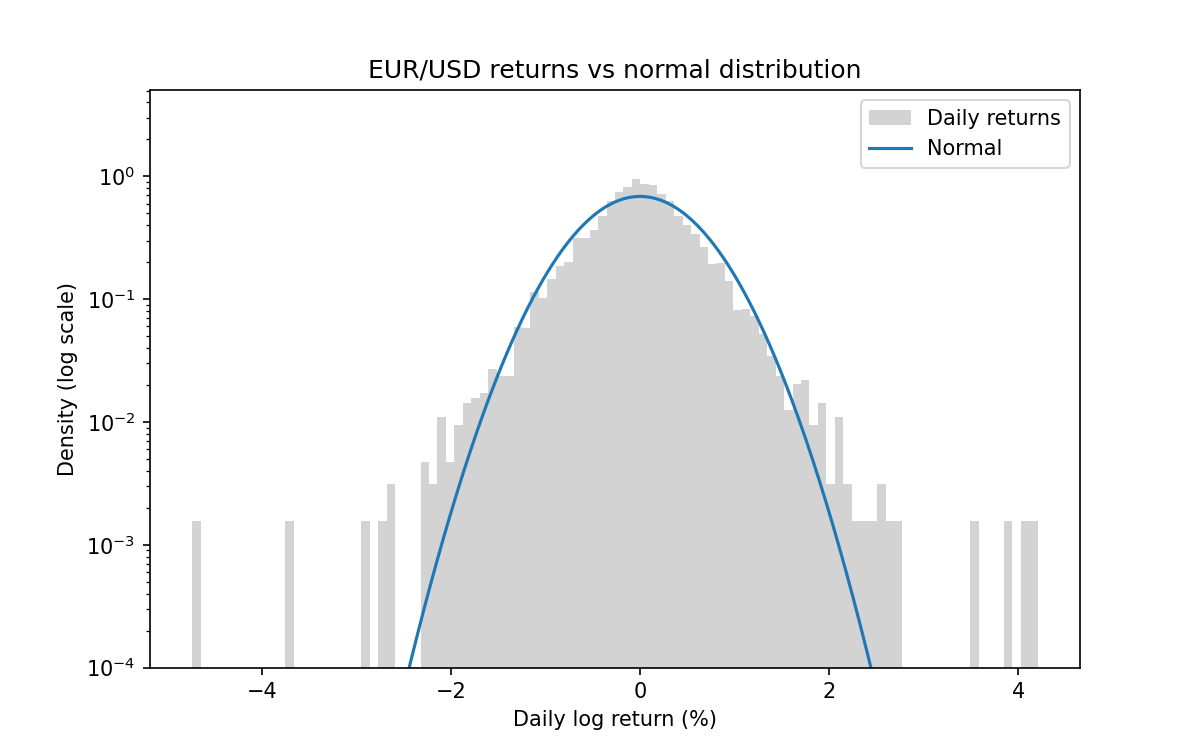
\includegraphics[width=0.8\textwidth]{histogram.png}
  \caption{Histogram of daily EUR/USD log returns with a fitted normal
  curve. The y-axis is logarithmic so that the rare tail days are visible.
  In the tails, the bars stay above the normal curve: more extreme days
  than the normal predicts.}
  \label{fig:hist}
\end{figure}

\begin{figure}[ht]
  \centering
  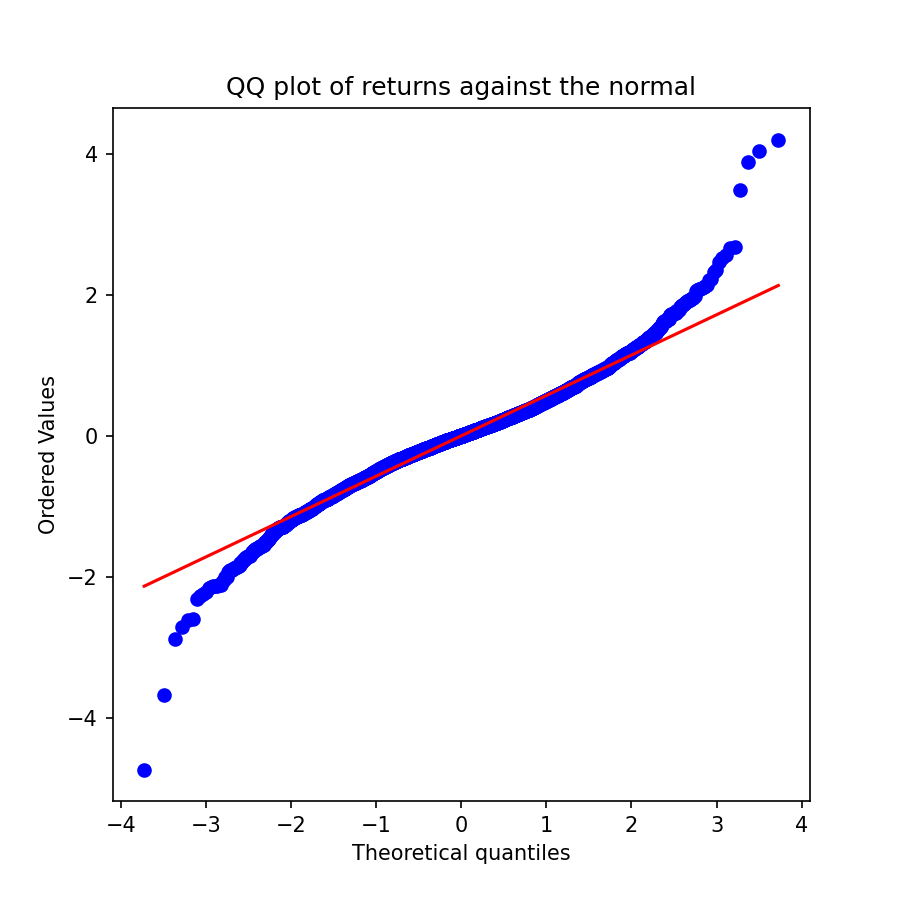
\includegraphics[width=0.55\textwidth]{qq_plot.png}
  \caption{QQ plot of the returns against a normal distribution. The middle
  follows the line; both ends bend away. That S-shape means fat tails.}
  \label{fig:qq}
\end{figure}

\begin{mistake}
Reading the histogram on a normal (not log) y-axis and saying ``it looks
like a bell curve''. In the middle it does. The difference is in the tails,
which are invisible on a normal axis. That is why the code uses
\code{plt.yscale("log")}.
\end{mistake}

\subsection{Step 3: Three ways to compute VaR}

For each day, the script looks at the 500 returns before it and computes:

\begin{enumerate}
  \item \textbf{Normal:} $-(\mu + z\sigma)$ with the window's $\mu$ and
    $\sigma$.
  \item \textbf{Historical:} minus the 1\% (or 5\%) quantile of the 500
    returns.
  \item \textbf{Monte Carlo normal:} 10{,}000 draws from a normal with the
    window's $\mu$ and $\sigma$, then minus the 1\% (or 5\%) quantile.
\end{enumerate}

All three methods are standard \citep{jorion2007}.

\begin{example}[: one window, two methods]
Suppose a 500-day window has $\mu=0$ and $\sigma=0.55\%$.
\begin{itemize}
  \item Normal 99\% VaR $= 2.326 \times 0.55 = 1.28\%$.
  \item Suppose the 5th worst return in the window is $-1.45\%$. Then the
    historical 99\% VaR is about $1.45\%$.
\end{itemize}
If the tails are fat, the historical number is larger. That is exactly the
pattern in the project.
\end{example}

\subsection{Step 4: The rolling backtest without look-ahead}

The loop runs from day 500 to the last day. Every day:

\begin{enumerate}
  \item Take \code{window = returns[day - 500:day]}. This stops just
    \emph{before} \code{day}, so today's return is not in it.
  \item Compute the six VaR numbers (3 methods $\times$ 2 levels).
  \item Later, compare today's real return with each VaR.
\end{enumerate}

That gives $7108 - 500 = 6608$ test days. Figure~\ref{fig:varlines} shows
the result for the 99\% level.

\begin{figure}[ht]
  \centering
  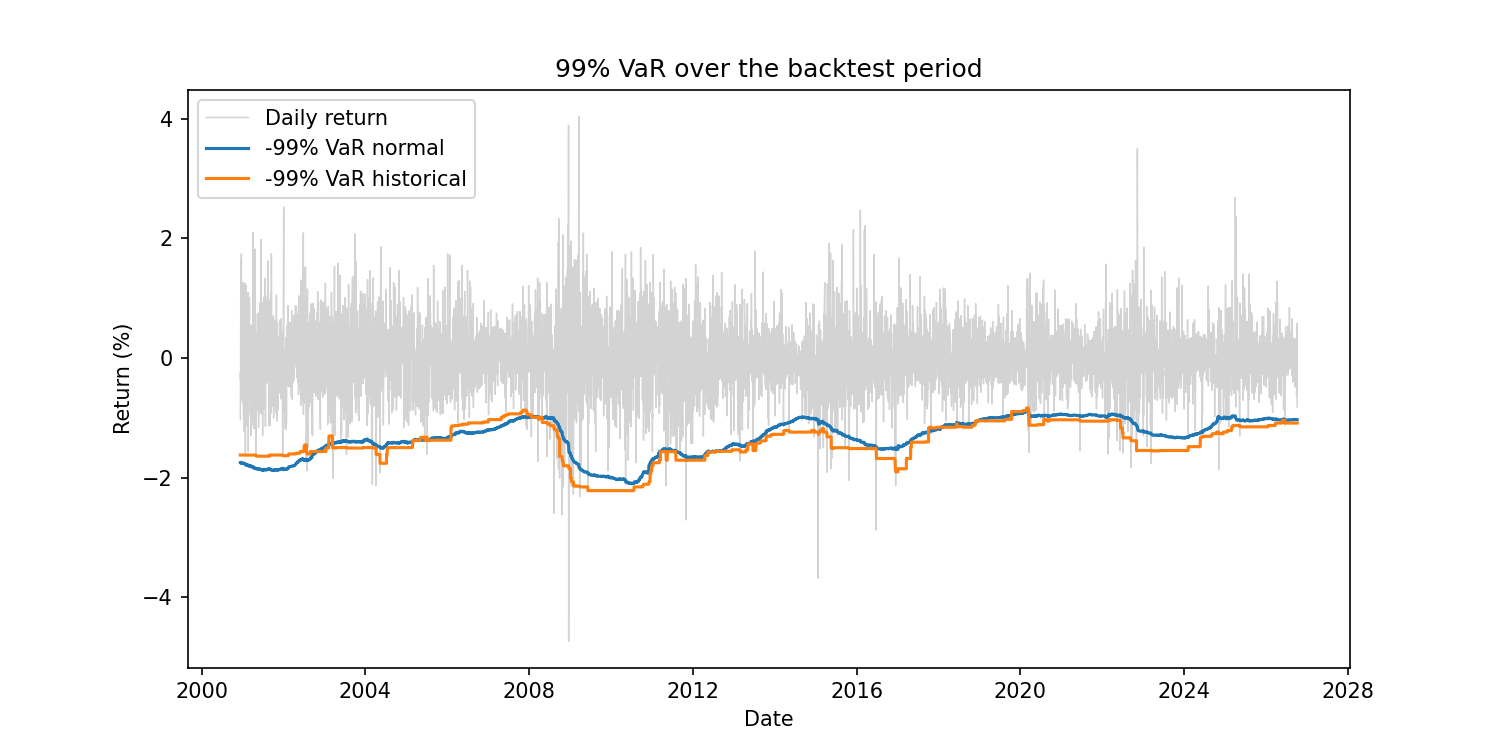
\includegraphics[width=\textwidth]{var_lines.png}
  \caption{Daily returns (grey) and minus the 99\% VaR for the normal and
  historical methods. Every grey spike below a line is an exceedance for
  that method. Note the wider grey band in 2008--2009: volatility
  clustering.}
  \label{fig:varlines}
\end{figure}

\subsection{Step 5: Counting exceedances and the Kupiec test}

These are the main results.

\begin{center}
\begin{tabular}{llrrr}
\toprule
Method & Level & Exceedances & Expected & Kupiec p-value \\
\midrule
Normal         & 95\% & 302 & 330.4 & 0.1040 \\
Historical     & 95\% & 324 & 330.4 & 0.7171 \\
Monte Carlo    & 95\% & 302 & 330.4 & 0.1040 \\
\midrule
Normal         & 99\% & 114 & 66.1 & 0.0000 \\
Historical     & 99\% &  74 & 66.1 & 0.3367 \\
Monte Carlo    & 99\% & 114 & 66.1 & 0.0000 \\
\bottomrule
\end{tabular}
\end{center}

Average 99\% VaR over the backtest: normal $1.32\%$, historical $1.41\%$.

\textbf{How to read the table, row by row.}
\begin{itemize}
  \item \textbf{95\%, all methods pass.} The normal model has 302 breaks
    when 330 were expected; p $= 0.10$, above 0.05. So the Kupiec test does
    not reject the 95\% VaR of the normal model. This only says the
    \emph{frequency} of breaks is consistent with 5\%. It does not mean that
    returns are normal; the Jarque--Bera test above rejects that strongly.
  \item \textbf{99\%, normal fails.} 114 breaks instead of 66 is about
    \emph{1.7 times} too many. The Kupiec statistic is about 28.8, far above
    3.84, so p $< 0.001$. The normal model underestimates risk deep in the
    tail.
  \item \textbf{99\%, historical passes.} 74 breaks against 66 expected,
    p $= 0.34$. No evidence against it.
  \item \textbf{Monte Carlo = normal.} Same assumption, so very close results (identical counts in this run).
\end{itemize}

\begin{onesentence}
The normal distribution is good enough in the ``ordinary bad day'' zone
(95\%), but too optimistic in the ``really bad day'' zone (99\%), because
EUR/USD has fat tails.
\end{onesentence}

\begin{example}[: why 99\% and not 95\%?]
Under a normal, the 95\% cutoff is $1.645\sigma$ and the 99\% cutoff is
$2.326\sigma$. Fat tails mean there is extra probability far out. At
$1.645\sigma$ you are not yet ``far out'', so the extra probability
barely shows. At $2.326\sigma$ you are, so it shows clearly.
\end{example}

\begin{mistake}
Saying ``the historical method is correct''. Passing Kupiec means ``not
rejected'', not ``right''. Historical simulation has its own problems
\citep{pritsker2006}, and the project does not test whether its breaks come
in clusters \citep{christoffersen1998}.
\end{mistake}

\subsection{Step 6: Scenario analysis to 2040 (bootstrap)}

The last part of the script asks: ``If the future days look like the past
days, what range of EUR/USD rates could we see at the end of 2040?''

\begin{enumerate}
  \item Start at the last rate, 1.1177.
  \item Count the working days left until 31 December 2040 (about 3700).
  \item For each of 5000 paths, draw that many daily returns at random from
    the 7108 historical returns, with replacement (bootstrap).
  \item Add up the log returns along each path and turn them back into
    rates, \[P_T = P_0 \exp\!\big(\textstyle\sum r_t / 100\big).\]
  \item At each future day, take the 5th, 50th and 95th percentile over the
    5000 paths.
\end{enumerate}

\begin{figure}[ht]
  \centering
  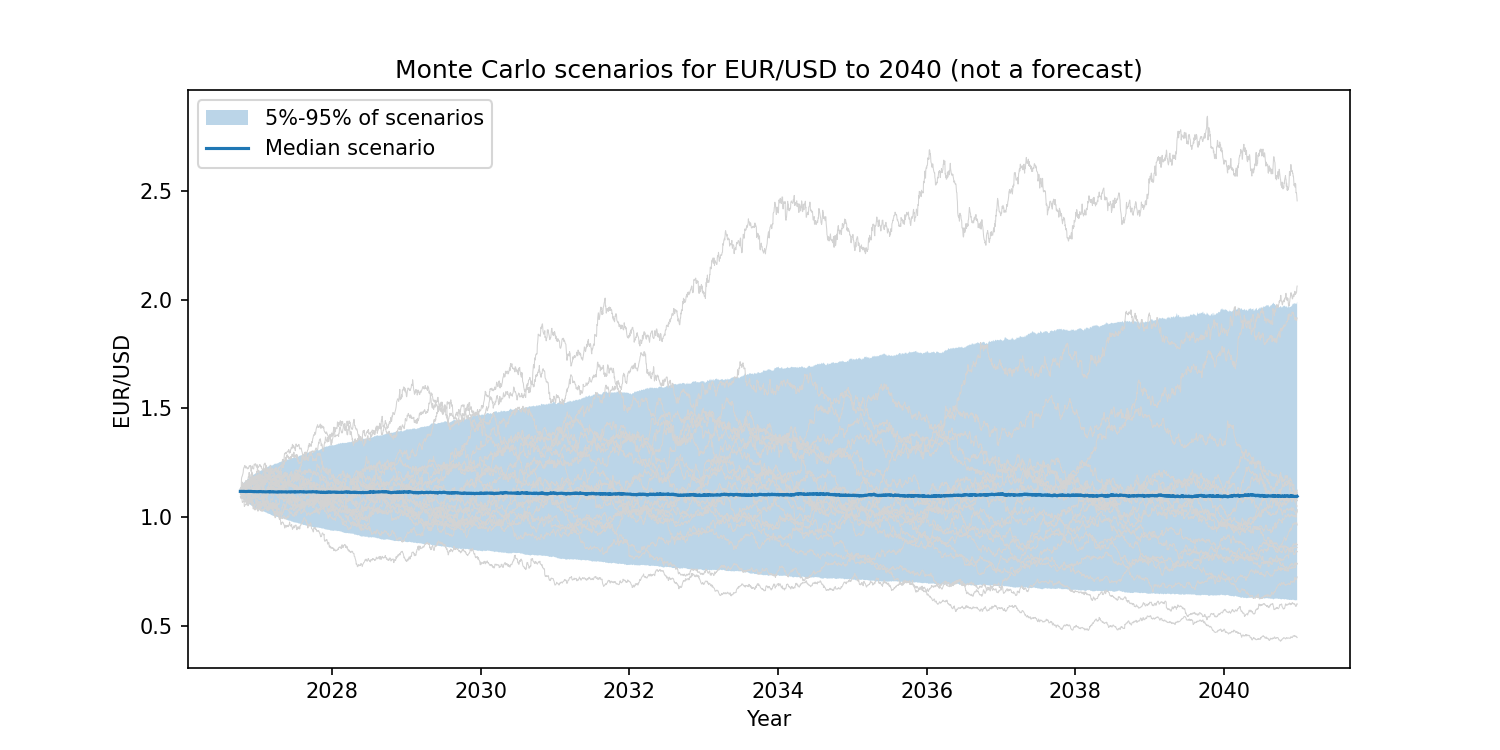
\includegraphics[width=\textwidth]{fan_2040.png}
  \caption{5000 bootstrap scenarios for EUR/USD to the end of 2040. Grey:
  20 example paths. Shaded: the 5--95\% band. Line: the median. This is a
  scenario analysis, not a forecast.}
  \label{fig:fan}
\end{figure}

Result at the end of 2040, \emph{under the bootstrap model} (not a
validated forecast interval for the real rate): 5th percentile about $0.62$, median about
$1.10$, 95th percentile about $1.99$.

\begin{example}[: a back-of-the-envelope check]
Daily $\sigma \approx 0.58\%$, about 3700 days. If days are independent,
the standard deviation of the \emph{sum} grows with the square root of
time: $0.58 \times \sqrt{3700} \approx 35\%$. A 90\% band is about
$\pm 1.645 \times 35\% \approx \pm 58\%$ in log terms. Then
$1.1177 \cdot e^{-0.58} \approx 0.63$ and $1.1177 \cdot e^{+0.58} \approx
2.00$. Very close to the simulated 0.62 and 1.99. (The small mean of
$-0.0008\%$ per day adds up to about $-3\%$ over 3700 days, which pulls
the median a little below the start rate.)
\end{example}

\textbf{Why this is not a forecast (my own reasoning).}
\begin{itemize}
  \item The model has no view on direction. The average return is about
    zero, so the median path stays near today's rate. That is not a
    prediction that ``the euro will stay at 1.10''; it is what happens when
    you have no information about direction.
  \item The width of the band is the message: anything from about 0.6 to
    about 2.0 is inside the 90\% band. That is a statement about
    uncertainty, not about a likely outcome.
  \item It only re-uses 1999--2026. A new kind of event cannot appear.
  \item Even serious economic models struggle to forecast exchange rates
    better than a random walk \citep{meese1983,rossi2013}. A simple
    bootstrap should not claim to do better.
\end{itemize}

\begin{mistake}
Showing the fan chart and saying ``the model predicts EUR/USD at 1.10 in
2040''. The model predicts nothing. It shows how wide the range of
possibilities is.
\end{mistake}

%=====================================================================
\section{Part C: How currency exchange rates vary with macroeconomic
trends}\label{sec:macro}
%=====================================================================

\begin{center}
\fbox{\parbox{0.9\textwidth}{\centering\small
This part is educational. The trading story is fictive and all numbers in
the orange boxes are made up. Nothing here is investment advice or a view on
where EUR/USD is going.}}
\end{center}

Part B treated EUR/USD returns as random numbers. But behind the numbers
are real economies: interest rates, inflation, central banks and fear.
Textbooks on exchange rate economics cover all of this in depth
\citep{sarnotaylor2003}.
Here is a short tour, built on one fictive scenario.

\begin{fictive}
We run a small (imaginary) FX trading desk. We hold a position in EUR/USD:
we own euros and count our profit in dollars. Today EUR/USD is
\textbf{1.10}. Our job is to understand what could move the rate, and to
be honest about how little we can predict.
\end{fictive}

\subsection{Interest rate differentials and interest rate parity}

\textbf{Idea.} Money likes to earn interest. If dollar deposits pay more
than euro deposits, investors are tempted to move money into dollars.

\textbf{Interest rate parity} says that, in theory, you cannot get a free
lunch from the interest gap. There are two versions:

\begin{itemize}
  \item \textbf{Covered parity:} if you lock in the future exchange rate
    today with a forward contract, the interest gap is cancelled by the gap
    between the forward rate and today's rate.
  \item \textbf{Uncovered parity (UIP):} without a forward contract, the
    high-interest currency is \emph{expected} to weaken by about the
    interest gap. With EUR/USD $=S$ (dollars per euro):
    \[
      \text{expected \% change in } S \;\approx\; i_{\text{USD}} - i_{\text{EUR}} .
    \]
\end{itemize}

\begin{fictive}
Dollar interest is 5\% a year and euro interest is 3\%. UIP says the euro
should be expected to \emph{rise} by about 2\% over the year
(from 1.10 to about 1.122), so that euro holders, who earn 2\% less
interest, are compensated by the currency gain. Then the total return is
the same in both currencies.
\end{fictive}

\textbf{What the data say.} UIP often does not hold in the data. The
forward rate turns out to be a biased guess of the future spot rate
\citep{fama1984}. So ``high interest rate = currency will weaken'' is a
theory benchmark, not a trading rule.

\begin{mistake}
Mixing up ``what happens on the day rates change'' and ``what UIP says
afterwards''. They can point in opposite directions. See overshooting below.
\end{mistake}

\subsection{Inflation and purchasing power parity (PPP)}

\textbf{Idea.} The same basket of goods should cost about the same in two
places after converting the currency. If prices in the US rise faster than
in the euro area, each dollar buys less, so over time you should need more
dollars per euro.

\textbf{Absolute PPP} says a basket costs the same in both places after
conversion, $S = P_{\text{US}} / P_{\text{EA}}$. \textbf{Relative PPP} is the
weaker, more used version about \emph{changes}:
\[
  \text{\% change in } S \;\approx\; \pi_{\text{US}} - \pi_{\text{EA}},
\]
where $\pi$ is inflation.

\begin{fictive}
US inflation is 4\% a year, euro area inflation is 2\%. Relative PPP says
EUR/USD should drift up by about 2\% a year: from 1.10 to about 1.12 after
one year, and further after that.
\end{fictive}

\textbf{What the data say.} PPP works poorly in the short run. Real exchange
rates swing a lot and move back towards PPP only slowly; this is called the
``PPP puzzle'' \citep{rogoff1996}. Whether PPP holds in the long run has
been debated for a long time \citep{taylortaylor2004}. For a daily VaR,
inflation hardly matters; for a 14-year scenario to 2040 it could matter,
and our bootstrap ignores it.

\subsection{Central bank policy: ECB vs Fed}

The European Central Bank (ECB) sets interest rates for the euro area; the
Federal Reserve (Fed) sets them for the US. Their decisions change the
interest rate gap from the previous section, and markets react to news
about \emph{future} decisions too, not only to the decisions themselves.

\begin{fictive}
Before a Fed meeting, everyone expects the Fed to keep its rate unchanged.
Instead it raises the rate by 0.50 percentage points. The ECB does nothing.
The dollar interest rate is now more attractive than expected. In our story,
EUR/USD falls from 1.10 to 1.09 within minutes. Our euro position loses
about 0.9\%.
\end{fictive}

Two lessons from the story:
\begin{itemize}
  \item It is the \emph{surprise} that moves the price. A decision everyone
    expected is already in the price.
  \item One central bank meeting can produce a day in the tail of the
    distribution. Those days are part of why the tails are fat.
\end{itemize}

Researchers have tried to use central bank rules (``Taylor rules'', where the
interest rate depends on inflation and the output gap) to predict exchange
rates out of sample; one example is \citet{molodtsovapapell2009}. For a
broad survey of what does and does not predict exchange rates, see
\citet{rossi2013}.

\subsection{Dornbusch overshooting}

\citet{dornbusch1976} explained why exchange rates can jump \emph{more}
than seems reasonable. Goods prices are sticky: they change slowly. Exchange
rates are not: they change in seconds. So after a monetary policy shock,
the exchange rate takes the whole adjustment at first and goes too far
(overshoots), and then partly comes back as prices slowly catch up.

\begin{fictive}
(Dornbusch's own example is a monetary expansion. Our Fed hike is the
mirror image: a contractionary shock.)
Continue the Fed story. After the surprise hike, EUR/USD drops from 1.10 to
1.07 (the dollar jumps up). Over the next year it drifts back up to about
1.09. Notice how this fits UIP: the dollar now pays more interest, and after
the jump it is \emph{expected to weaken} slowly, which is exactly what UIP
asks for. The jump today makes room for the expected slow fall later.
\end{fictive}

\begin{onesentence}
Overshooting: the exchange rate moves too far at once because prices are
slow, then partly moves back.
\end{onesentence}

\subsection{Safe-haven demand for the US dollar}

\textbf{Idea.} When markets are scared, investors sell risky assets and buy
what they see as safe. Some currencies tend to gain in such stress
episodes; they are called safe-haven currencies
\citep{ranaldosoderlind2010}. \citet{habib2012} study what makes a currency
a safe haven. The US dollar has a special role as the world's main reserve
currency \citep{maggiori2017}.

\begin{fictive}
A sudden global financial panic starts. In our story, investors around the
world buy US dollars and US government bonds. EUR/USD falls from 1.10 to
1.05 in two weeks, even though nothing changed in euro area interest rates
or inflation. Our euro position loses about 4.7\%. The fall had nothing to
do with ``fundamentals'' in the textbook sense. It came from fear.
\end{fictive}

This is also a link back to Part B: stress periods are where volatility
clusters and where fat-tail days live. A VaR model built on calm years will
be surprised by them.

\subsection{The honest message: models struggle to beat a random walk}

After all this theory, the most important result in the field is a humble
one. \citet{meese1983} compared economic exchange rate models with a simple
random walk (``tomorrow = today'') and found that the models did not beat
it out of sample. Later work shows that this is still a hard benchmark to
beat, although predictability has been found for some models, samples and
forecast horizons \citep{rossi2013,molodtsovapapell2009}. \citet{engelwest2005} give one explanation: even if
exchange rates are driven by fundamentals like interest rates and money
supply, they can still look almost like a random walk.

\begin{fictive}
Our trading desk builds a beautiful model with interest rates, inflation and
central bank signals. On past data it ``explains'' a lot. But when we test
it on new data, it guesses tomorrow's EUR/USD no better than just using
today's rate. This can well happen: the random walk is a very hard
benchmark to beat.
\end{fictive}

What this means for the project (my own reasoning):
\begin{itemize}
  \item It is reasonable that the project models \emph{risk} (how big the
    moves can be) and not \emph{direction} (which way they go). Risk is
    the part we can measure with some confidence.
  \item It is also why the 2040 fan chart is a scenario analysis: if expert
    models cannot reliably beat ``tomorrow = today'', a bootstrap of past
    returns should not pretend to know 2040.
\end{itemize}

\begin{onesentence}
Macro forces clearly move exchange rates, but turning them into reliable
forecasts is very hard, so the project measures risk instead of predicting
direction.
\end{onesentence}

%=====================================================================
\section{Limitations}\label{sec:limits}
%=====================================================================

Every project has limits. Saying them clearly is part of the result.

\begin{enumerate}
  \item \textbf{Independent days in the bootstrap.} Every future day is
    drawn on its own. In real data, calm days cluster and wild days cluster.
    The bootstrap mixes a 2008 day next to a quiet 2014 day, so long stormy
    spells are probably too rare in the scenarios.
  \item \textbf{Volatility clustering is ignored in the VaR.} The 500-day
    window gives equal weight to a day two years ago and yesterday. After a
    sudden shock the VaR reacts slowly. A GARCH model
    \citep{bollerslev1986} would react faster. The Kupiec test also does not
    check if exceedances cluster \citep{christoffersen1998}.
  \item \textbf{Only 1999--2026 history.} The bootstrap and the historical
    VaR can only produce moves that happened in that period. A shock bigger
    than the worst day so far is impossible in the model.
  \item \textbf{One currency pair.} EUR/USD is the most traded pair and may
    behave differently from smaller currencies. Results for EUR/SEK or
    EUR/CHF could be different.
  \item \textbf{No costs.} No bid/ask spread, no trading fees, no interest
    from holding the currencies. A real position would earn or pay
    interest every day.
  \item \textbf{One snapshot per day.} The ECB rate is a snapshot in the
    early afternoon. Moves inside the day are invisible.
  \item \textbf{Calendar detail.} The scenario counts 261 weekdays per year,
    a little more than the number of ECB working days, so the 2040 band
    is very slightly wider than it would otherwise be.
\end{enumerate}

%=====================================================================
\section{Exercises}\label{sec:exercises}
%=====================================================================

Try them before you look at the answers.

\begin{enumerate}[label=\textbf{\arabic*.}]
  \item Prices are 1.20, 1.26, 1.197. Compute the two daily log returns in
    percent and their sum. What is $100\ln(1.197/1.20)$?
  \item EUR/USD goes from 1.15 to 1.13. Did the euro or the dollar get
    stronger? Is the return positive or negative?
  \item SciPy says excess kurtosis $= 0.1$. Is the distribution's kurtosis
    close to that of a normal?
  \item $n=1200$, $S=0.2$, $K=0.5$. Compute the Jarque--Bera statistic. Is
    normality rejected at 5\% (critical value 5.99)?
  \item A window has $\mu = 0.01\%$ and $\sigma = 0.70\%$. Compute the 95\%
    and the 99\% normal VaR.
  \item A 99\% VaR is tested on 2000 days. How many exceedances do you
    expect? You see 40. Is that likely to be a problem?
  \item A friend writes \code{window = returns[day - 500:day + 1]}. What is
    wrong?
  \item Why does the Monte Carlo VaR in the project give the same number of
    exceedances as the normal VaR?
  \item Name two reasons why the 2040 fan chart is not a forecast.
  \item In the fictive story, US inflation is 3\% and euro area inflation is
    3\%. What does relative PPP say about EUR/USD?
\end{enumerate}

\subsection*{Short answers}

\begin{enumerate}[label=\textbf{\arabic*.}]
  \item $100\ln(1.26/1.20) = +4.88\%$, $100\ln(1.197/1.26) = -5.13\%$. Sum
    $= -0.25\%$, which equals $100\ln(1.197/1.20) \approx -0.25\%$. Log
    returns add up.
  \item The rate fell, so one euro buys fewer dollars: the dollar got
    stronger, the euro weaker. The return is negative:
    $100\ln(1.13/1.15) \approx -1.75\%$.
  \item Yes. Kurtosis $= 3 + 0.1 = 3.1$, close to the normal's 3.
  \item $JB = \frac{1200}{6}(0.04 + 0.25/4) = 200 \times 0.1025 = 20.5 >
    5.99$. Rejected.
  \item 95\%: $-(0.01 - 1.645 \times 0.70) = 1.14\%$.
    99\%: $-(0.01 - 2.326 \times 0.70) = 1.62\%$.
  \item Expected $0.01 \times 2000 = 20$. Seeing 40 is double. The Kupiec
    test rejects clearly (LR is about 15, far above 3.84). The VaR is too
    low.
  \item The slice now includes \code{returns[day]}, the return being
    tested. That is look-ahead bias.
  \item It draws from a normal distribution with the same $\mu$ and
    $\sigma$. With 10{,}000 draws the simulated quantile is almost the
    formula quantile. Same assumption, same thin tails.
  \item The model has no view on direction (mean about zero); it only
    re-uses the past; and exchange rates are known to be very hard to
    forecast \citep{meese1983,rossi2013}.
  \item The inflation gap is zero, so PPP gives no reason for the rate to
    drift in either direction.
\end{enumerate}

%=====================================================================
\newpage
\section{Cheat sheet}\label{sec:cheat}
%=====================================================================

\begin{center}
\renewcommand{\arraystretch}{1.6}
\begin{tabular}{p{0.28\textwidth}p{0.64\textwidth}}
\toprule
\textbf{What} & \textbf{Formula / rule} \\
\midrule
EUR/USD quote & 1 euro costs $S$ dollars. $S$ up $=$ euro stronger $=$
  positive return. \\
Log return (\%) & $r_t = 100\ln(P_t/P_{t-1})$ \\
Back to a price & $P_T = P_0 \exp\!\big(\sum_t r_t/100\big)$ \\
Mean & $\mu = \frac{1}{n}\sum r_t$ \\
Standard deviation & $\sigma = \sqrt{\frac{1}{n}\sum (r_t-\mu)^2}$ \\
Square-root-of-time & $\sigma_{T\text{ days}} \approx \sigma_{\text{1 day}}\sqrt{T}$
  (independent days) \\
Excess kurtosis & kurtosis $-\,3$ (normal: 0) \\
Jarque--Bera & $JB = \frac{n}{6}\left(S^2 + \frac{K^2}{4}\right) \sim
  \chi^2(2)$; 5\% critical value 5.99 \\
Normal VaR & $\text{VaR} = -(\mu + z\sigma)$, $z = \Phi^{-1}(1-\text{level})$ \\
$z$ values & 95\%: $-1.645$ \quad 99\%: $-2.326$ \\
Historical VaR & $-\,$quantile$_{1-\text{level}}$ of past returns \\
Exceedance & $r_t < -\text{VaR}_t$ \\
Expected exceedances & $(1-\text{level}) \times n$ \\
Kupiec LR & $-2\ln\!\left[\dfrac{(1-p)^{n-x}p^{x}}
  {(1-\frac{x}{n})^{n-x}(\frac{x}{n})^{x}}\right] \sim \chi^2(1)$;
  5\% critical value 3.84 \\
ARCH(1) & $\sigma_t^2 = \omega + \alpha\varepsilon_{t-1}^2$ \\
GARCH(1,1) & $\sigma_t^2 = \omega + \alpha\varepsilon_{t-1}^2 +
  \beta\sigma_{t-1}^2$ \\
UIP & expected \% change in $S \approx i_{\text{USD}} - i_{\text{EUR}}$ \\
Relative PPP & \% change in $S \approx \pi_{\text{US}} - \pi_{\text{EA}}$ \\
\midrule
p-value rule & p $< 0.05$: reject $H_0$. p $\ge 0.05$: no evidence against
  $H_0$ (not proof). \\
Project results & JB $= 3243.9$; 99\%: normal 114 vs 66.1 (rejected),
  historical 74 (p $=0.34$); 95\%: both pass. \\
\bottomrule
\end{tabular}
\end{center}

%=====================================================================
\newpage
\bibliographystyle{plainnat}
\bibliography{references}

\end{document}
